\documentclass[11pt,a4paper]{report}

\usepackage[utf8]{inputenc}
\usepackage[T1]{fontenc}

%%%%%%%%%%% Own packages
\usepackage[a4paper, margin=1in]{geometry}
\usepackage{multicol}

% Boxing
\usepackage[most]{tcolorbox}
\tcbset{enhanced}
%\usepackage{capt-of}	% captions in boxes

% Header/footer
\usepackage{fancyhdr}
\pagestyle{fancy}
\renewcommand{\headrulewidth}{0pt}

% Listsings and items
\usepackage{enumerate}
\usepackage{varioref}
\usepackage{hyperref}
\usepackage{cleveref}

% Maths
\usepackage{physics}
\usepackage{cancel}
\usepackage{amstext,amsbsy,amssymb}
\usepackage{times} 
\usepackage{siunitx}

%% Graphics
\usepackage{caption}
\captionsetup{margin=10pt,font=small,labelfont=bf}
%\renewcommand{\thesubfigure}{(\alph{subfigure})} % Style: 1(a), 1(b)
%\pagestyle{empty}
\usepackage{graphicx}% Include figure files
%\usepackage{epstopdf}
%\usepackage{pdfsync}


%% Numbered problems
\newcounter{excount}[chapter]
\newenvironment{exercise}[1][]{\addtocounter{excount}{1} \noindent {\bf Problem
    \arabic{excount} \ \ #1}\hspace{2mm}}{\vspace{4mm}}

%% Solution environment
\newenvironment{solution}
    {\begin{tcolorbox}[title=Solution,halign lower=right,breakable]
    }
    {
    \tcblower Jakob Borg
    \end{tcolorbox}
	\vspace{5mm}
    }

%% Figure command
\newcommand{\fig}[2][]
{
\begin{center}
\includegraphics[width=0.49\linewidth]{#2}
\captionof{figure}{#1}
\label{fig:fig\arabic{figure}}
\end{center}
}

%% Quic-half
\newcommand{\half}
{
\frac{1}{2}
}

%% Quick center-of-mass
\newcommand{\com}
{
\text{c.m.}
}

%% quad while
\newcommand{\qwhile}
{
\qq{while}
}

%% Lagrangian's equation
\newcommand{\Leq}[1]
{
\dv{t}\qty(\pdv{L}{\dot{#1}}) - \pdv{L}{#1}
}

%% Quick L pdv
\newcommand{\Lpdv}[1]
{
\pdv{L}{#1}
}

%% Time derivative of Lpdv
\newcommand{\dvtLpdv}[1]
{
\dv{t} \qty(\Lpdv{#1}) 
}

%% Time derivative of argument
\newcommand{\dvt}[1]
{
\dv{t} \qty(#1)
}

%% Quick theta dot and phi dot
\newcommand{\dtheta}
{
\dot{\theta}
}
\newcommand{\dphi}
{
\dot{\phi}
}
\newcommand{\ddtheta}
{
\ddot{\theta}
}
\newcommand{\ddphi}
{
\ddot{\phi}
}

%% Quick sin cos of theta and phi commands
\newcommand{\cost}
{
\cos(\theta)
}
\newcommand{\sint}
{
\sin(\theta)
}
\newcommand{\cosp}
{
\cos(\phi)
}
\newcommand{\sinp}
{
\sin(\phi)
}

\title{FYS3120 Classical Mechanics and Electrodynamics\\ 
\vspace{15mm}Problem set 3}
\author{Jakob Borg}
\date{7 February, 2019}
%%%%%%%
\begin{document}
%%%%%%%

\maketitle

%\lhead{Jakob Borg}
\lhead{Problem set 3 FYS3120}
\rhead{Jakobbor}
%%%%%%%%


%%%%%%%%
\begin{exercise}
An object with mass $m$ slides without friction on a plane inclined 30$^\circ$. The plane is forced to move horizontally with a constant acceleration $a$. In this case a natural choice of generalized coordinate will be the displacement $s$ of the object along the tilted surface. See Fig.~\ref{fig:fig1} for an illustration.

\begin{itemize}
\item[\bf a)] Assume first the inclined plane to be at rest, with vanishing velocity and acceleration. Express the Cartesian coordinates $x,y$ of the sliding object as functions of $s$. Find the Lagrangian expressed in terms of $s$ and $\dot s$.
\item[\bf b)]  Assume next the acceleration $a$ to be constant and non-vanishing. Again find the Cartesian coordinates, and their time derivatives, expressed in terms of $s$ and $\dot s$, and determine the Lagrangian.
\item[\bf c)] Find Lagrange's equation for the system, and solve the equation under the assumption that the body starts at time $t=0$ from the top of the inclined plane ($s=0$) with zero velocity relative to the plane.
\end{itemize}
\begin{solution}
\fig[Motion on an inclined accelerated plane.]{./figurer/{figurer.001}.png}
\begin{enumerate}[\bf a)]

\item With the incline at rest, this is just like a normal box sliding down an incline. I assume the box to move in the plane so I need $x$ and $y$ coordinates. With one constraint on the vertical position, so $ d = 2\cdot 1 - 1 = 1$ d.o.f. Here I would like to remind both myself and the reader that $\theta$ is not a coordinate. I find the Cartesian coordinates
\begin{align*}
\cost = \frac{x}{s} \quad  &\Rightarrow \quad x = s\cost
\\
\tan(\theta) = \frac{h-y}{x}  \quad &\Rightarrow \quad  y = h - x \tan(\theta) = h- s\sint
\end{align*}
The Lagrangian in the generalized coordinates
\begin{gather*}
L = K-V \qc V = mgy = mg\qty( h-s\sint)
\\
K = \half m\dot{\va{r}}^2 = \half m \qty( \dot{x}^2 + \dot{y}^2 ) = \half m \qty( \dot{s}^2 \cos[2](\theta) + \dot{s}^2\sin[2](\theta)) = \half m\dot{s}^2
\\
L = \half m\dot{s}^2 - mg\qty(h-s\sint)
%\\
%\dv{t}\qty( \Lpdv{\dot{s}}) = \dv{t}\qty( m\dot{s} ) = m\ddot{s}
%\\
%\Lpdv{s} = mg\sint
%\\
%m\ddot{s} -mg\sint = 0
\end{gather*}

\item With the incline moving with constant acceleration $a$, the x-position of the box is shifted along with the movement. Let $X_a$ be the position of the incline. The Cartesian coordinates
\begin{align*}
\cost = \frac{x - x_A}{s} \quad &\Rightarrow \quad x =  s\cost + X_a = s\cost + \half a t^2
\\
\tan(\theta) = \frac{h-y}{x-X_a} \quad &\Rightarrow \quad y = h-\qty(x-X_a)\tan(\theta) = h-s\sint
\end{align*}
The y-coordinate is unchanged, and so is the potential energy and its time derivative. I find the kinetic energy and the Lagrangian
\begin{gather*}
\dot{x}^2 = \qty( \dot{s}\cost + at ) ^2 = \dot{s}^2\cos[2](\theta) + 2\dot{s}\cost at + a^2t^2
\\
K = \half m\qty( \dot{x}^2 + \dot{y}^2 ) = \half m \qty( \dot{s}^2\cos[2](\theta) + 2\dot{s}\cost at + a^2t^2 + \dot{s}^2\sin[2](\theta) )
\\
= \half m \qty( \dot{s}^2 + 2\dot{s}\cost at + a^2t^2)
\\
L = \half m \qty( \dot{s}^2 + 2\dot{s}\cost at + a^2t^2) - mg\qty( h-s\sint)
\end{gather*}

\item With one coordinate there is only one Lagrange equation
\begin{gather*}
\Leq{s} = 0
\\
\dv{t}\qty( \Lpdv{\dot{s}} ) = \dv{t}\qty( m\dot{s} + m\cost at ) = m\ddot{s} + m\cost a \qc \Lpdv{s} = mg\sint
\\
m\ddot{s} + m\cost a - mg\sint = 0
\\
\qq{giving the differential equation:}
\\
\ddot{s} = g\sint - \cost a
\end{gather*}
where all the terms on the right hand side are constants, let $g\sint - \cost a = \kappa$. This equations has a power law solution on the form $s = \half \kappa t^2 + v_0t + s_0$. Under the initial conditions given
\begin{align*}
s(0) = 0 \quad &\Rightarrow \quad s_0 = 0
\\
\dot{s}(0) = 0 \quad &\Rightarrow \quad v_0 = 0
\\
\qq*{giving the full solution} s &= \qty(g\sint - a \cost ) \frac{t^2}{2}
\end{align*}
\end{enumerate}
\end{solution}
\end{exercise}
%%%%%%%%%%


%%%%%%%%
\begin{exercise}
A rigid circular metal hoop rotates with constant angular velocity $\omega$ around an axis bisecting the hoop. A particle slides without friction along the hoop and there is no gravity. Use the angle $\theta$ with respect to the rotation axis as generalized coordinate (see Fig.~\ref{fig:fig2}).

\begin{itemize}
\item[\bf a)] Find the Lagrangian expressed in terms of $\theta$ and $\dot\theta$, and derive Lagrange's equation for this variable.
\item[\bf b)] Show that the Lagrangian is the same as the Lagrangian of a particle moving in a time-independent, periodic potential $V(\theta)$, with two stable and two unstable equilibrium points (within a $2\pi$ interval).
\item[\bf c)] With $\theta_0$ as one of the stable equilibrium points, introduce a small deviation, $\phi=\theta-\theta_0$, and determine the small-angle form of the equation of motion (keeping only the lowest order in $\theta$ and its derivative). What is the angular frequency of oscillations about the stationary point?
\end{itemize}
\begin{solution}
\fig[Rotating hoop.]{./figurer/{figurer.002}.png}
\begin{enumerate}[\bf a)]

\item With no gravity there are no potential energy. The kinetic energy of the particle can be decomposed into two rotational movements. One term around the hoop $\half m R^2 \dtheta^2$, and one term from the rotation of the hoop itself. I will assume the hoop to be massless, so that the rotation of the hoop can be modeled as the point mass orbiting with constant angular velocity $\omega$ in a radius $R\sint$ where $R$ is the radius of the hoop, giving kinetic energy $\half mR^2\sin[2](\theta)$.
\begin{gather*}
L = K = \half m \qty(R\sint)^2\omega^2 + \half mR^2\dtheta^2
\\
\dvtLpdv{\dtheta} = \dv{t}\qty( mR^2\dtheta ) = mR^2 \ddtheta
\\
\Lpdv{\theta} = mR^2\sint\cost w^2
\\
\qq*{giving Lagrange's equation} \ddtheta - \sint \cost \omega^2 = 0
\end{gather*}

\item By studying the Lagrangian I can see that it looks like kinetic energy of a point mass moving on a circle with constant radius $R$, and acted on by an effective potential $$U = - \half m R^2 \omega^2 \sin[2](\theta).$$ This will produce a Lagrangian $$L = K - U = \half mr^2\dtheta^2 +\half m R^2 \omega^2 \sin[2](\theta)$$ just like the Lagrangian from \textbf{a)} which originally only consisted of kinetic energies.

\item To find the equilibrium points I will look at where the derivative of the potential ${V\propto -\sin[2](\theta)}$, ${V' = -\sint\cost}$ is zero. Which is at ${\theta_0 = n\pi}$ and ${\theta_0 = m\frac{\pi}{2}}$ for $n = 0,1,2,\ldots$ and $m=1,3,5,\ldots$.
To find the stable equilibrium point I will just look at the plot of the potential $V=-\half \sin[2](\theta)$, and find that the ${\theta_0 = m\frac{\pi}{2}}$ are the stable ones. I choose to look at $\theta_0 = \frac{\pi}{2}$. Introducing small angle oscillations $\phi$ around $\theta_0$ I rewrite the e.o.m. as
\begin{gather*}
\ddphi -\omega^2\sin(\phi + \theta_0)\cos(\phi + \theta_0) = 0
\\
\ddphi - \omega^2 
\biggl(\cancel{\sinp \cos(\theta_0)} + \cosp\underbrace{\sin(\theta_0)}_{=1} \biggr)\biggl(\cancel{\cosp\cos(\theta_0)} - \sinp  \underbrace{\sin(\theta_0)}_{=1} \biggr)
= 0
\\
\ddphi + \omega^2 \cosp\sinp = 0
\end{gather*}
In the small angle approximation to the first order we have
\begin{align*}
\cosp = 1 - \mathcal{O}(\phi^2) \qc \sinp = \phi - \mathcal{O}(\phi^3)
\end{align*}
giving
\begin{align*}
\ddphi + \omega^2 \phi = 0
\end{align*}
which is the harmonic oscillator with angular frequency $\omega$.
\end{enumerate}
\end{solution}
\end{exercise}
%%%%%%%%


%%%%%%%%
\begin{exercise}
Two bodies with the same mass, $m$, are connected with a massless rope through a small hole in a smooth horizontal plane. One body is moving on the plane, the other one is hanging at the end of the rope and can move vertically. At all instances
the rope is tight. The acceleration due to gravity is $g$.

\begin{itemize}
\item[\bf a)] Find Lagrange's equations of motion in polar coordinates ($r,\theta$). 
%and explain their physical meaning. Discuss special cases.
\item[\bf b)] Reduce the equations of motion to a one dimensional problem in $r$ 
%with an effective potential 
and make a qualitative description of the motion. It can be helpful to solve the resulting differential equation numerically.
\end{itemize}

\begin{solution}
\fig[Two bodies connected by a rope through a small hole.]{./figurer/{figurer.003}.png}
\begin{enumerate}[\bf a)]
\item To describe the system in polar coordinates, I look at the system head on like in the right-most drawing. As I've indicated, let the hanging mass be body 1 and the other body 2.  Let the length of the rope be $l$.

In these coordinates the position of body 1 is simply ${\va{r}_1 = 0\vu{r} + 0\vu{\phi} = (0,0)}$. The position of body two is ${\vu{r}_2 = r\vu{r} + \phi \vu{\phi}}$. From the constraint of the length of the rope, I know the distance from the table down to body 1 to be $l-r$. 

The kinetic energy contributions are from the rotational and radial motion of body 2, and the vertical motion of body 1 which has the same velocity as the radial motion of body 2.
\begin{gather*}
K = 2\cdot \half m \dot{r}^2 + \half m r^2\dphi^2
\end{gather*}
Let the zero of the potential be at the height of the table, so that only body 1 contributes with potential energy
\begin{align*}
V = -mg(l-r)
\end{align*}
giving the Lagrangian
\begin{align*}
L = m\dot{r}^2 + \half m r^2 \dphi^2 + mg(l-r).
\end{align*}
I find the e.o.m. using Lagrange's equation $ \Leq{q_i} = 0$
\begin{multicols}{2}
\noindent
\begin{gather*}
\dvtLpdv{\dot{r}} = \dv{t}\qty( 2m\dot{r} ) = 2m\ddot{r}
\\
\Lpdv{r} = mr\dphi^2 -mg
\\
2\ddot{r} - r\dphi^2 + g = 0
\end{gather*}%
\begin{gather*}
\dvtLpdv{\dphi} = \dvt{mr^2\dphi} = 2mr\dot{r}\dphi + mr^2\ddphi
\\
\Lpdv{\phi} = 0 \qq{cyclic coordinate!} p_\phi = mr^2 \dphi 
\\
\ddphi + \frac{2}{r}\dot{r}\dphi= 0
\end{gather*}
\end{multicols}

\item As I've shown, $\phi$ is a cyclic coordinate with generalized momentum ${p_\phi = mr^2 \dphi }$. This reduces the d.o.f. by one, and I'm left with the e.o.m. from the $r$ coordinate. Here I can insert the expression for $\dphi$ from the generalized momentum
\begin{gather*}
2\ddot{r}-r\qty(\frac{p_\phi}{mr^2})^2 + g = 0 \quad
\Rightarrow \quad \ddot{r}- \frac{p_\phi^2}{2m^2}r^{-3} + \frac{g}{2} = 0
\end{gather*}
I will describe the system in terms of the position of body 2. First, if the system starts out with zero angular velocity the body will only slide from the initial position in to the center of the plane, accelerated by half as much as a body in free fall $\ddot{r} = -\half g$.

With initial angular velocity the body will start orbiting around the hole in the center. It can be shown that as the e.o.m. are dependent on $r^{-3}$ there are no stable circular orbits. The body will spiral in and out in a motion around the center. I've solved the e.o.m. numerically and plotted the position of body 2 around the center as well as the radial and angular component vs time in \cref{fig:simulations}. These are only one set of initial conditions with all variables and parameters set equal to one, except $\dot{r}=0.5$. Different initial conditions will have more or less spacing between each <<arm>> of the spiral, but they all share the spiral pattern. This movement is caused by the constant generalized momentum $p_\phi$, or the angular momentum in this case.
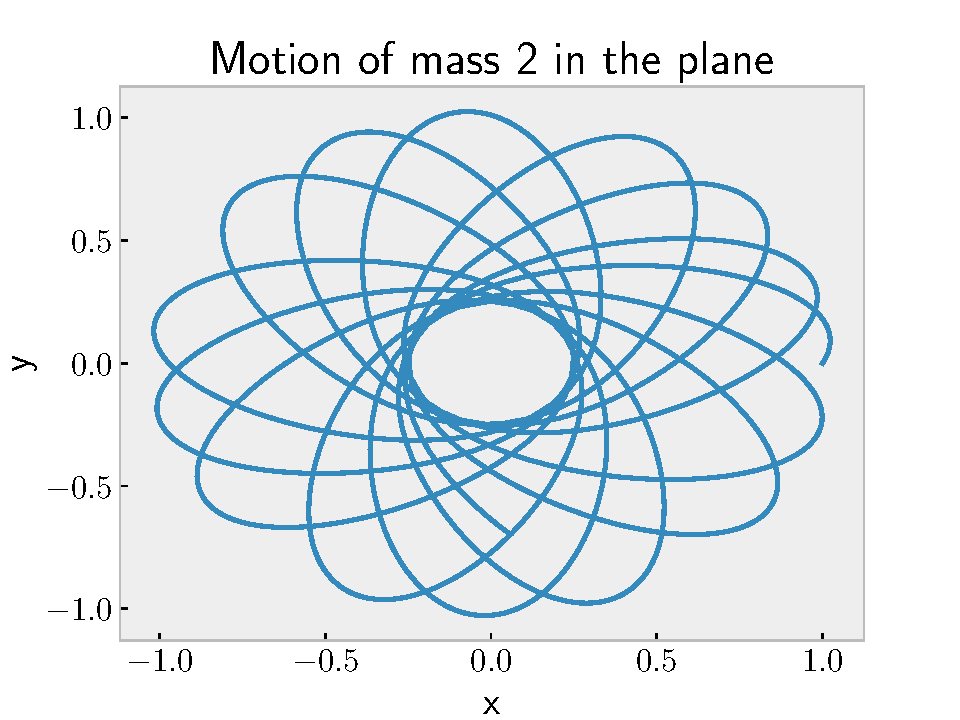
\includegraphics[width = 0.49\linewidth]{./figurer/polar_movement.pdf}
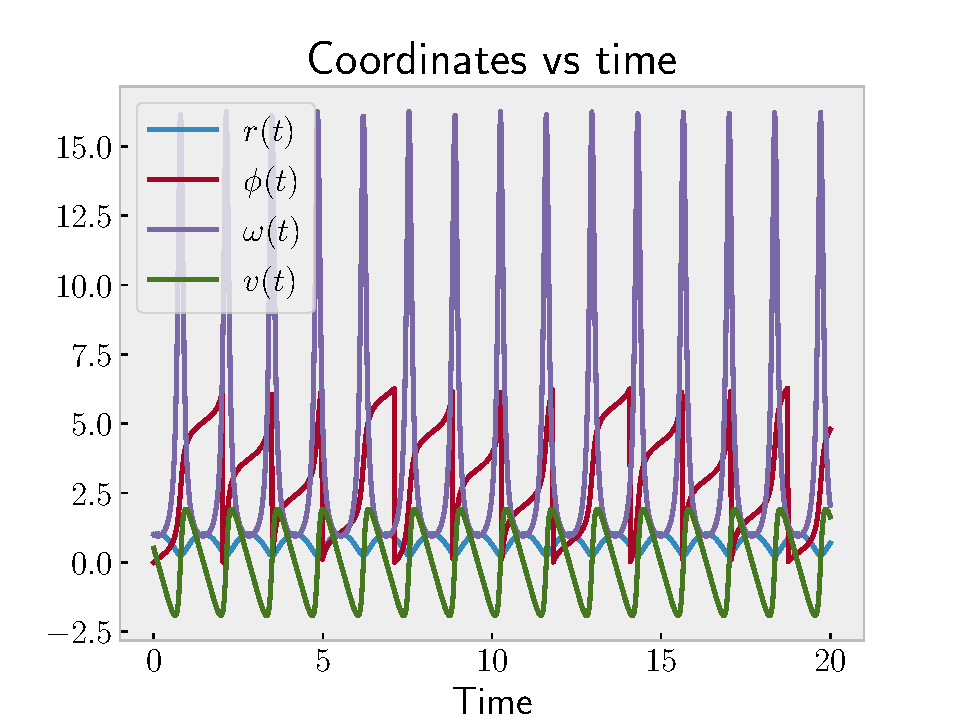
\includegraphics[width = 0.49\linewidth]{./figurer/components_vs_time.pdf}
\captionof{figure}{To the right, the motion of body 2 in the plane. Left, the radial and angular components as a function of time.}\label{fig:simulations}
\end{enumerate}
\end{solution}
\end{exercise}
%%%%%%%%


\end{document}

